\chapter{Comunicazione tra processi}
\thispagestyle{empty}

Occorre che i processi comunichino. Si parla di \textbf{IPC} - InterProcess Communication.

Ci sono tre questioni da considerare:
\begin{itemize}
    \item passaggio di informazioni.
    \item concorrenza nelle sezioni critiche.
    \item sequenzializzazione in presenza di dipendenze.
\end{itemize}

Le ultime due questioni sono applicabili anche ai thread.

\begin{wrapfigure}[5]{R}{40mm}
    \vspace{-5mm}
    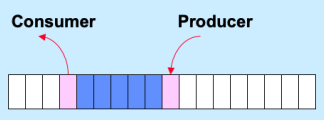
\includegraphics[width=50mm,height=25mm,keepaspectratio]{assets/producerconsumer6.png}
\end{wrapfigure}

Un famoso problema è quello del \textbf{produttore-consumatore} (\textit{bounded buffer problem}): due processi condividono un buffer comune di dimensione fissa, il produttore inserisce le informazioni, il consumatore le preleva. Il buffer ha due indici, uno per inserimento e uno per prelievo. Il problema che si viene a creare è la race condition, che può portare ad un deadlock, vedremo in seguito che significa.




\section{Corse critiche}
In alcuni sistemi i processi possono condividere una parte di memoria comune, che ciascuno può leggere e scrivere.

Situazioni nelle quali due processi stanno leggendo o scrivendo qualche dato condiviso, ed il risultato finale dipende dall'\textit{ordine} con cui vengono eseguiti i processi, prendono il nome di \textbf{race conditions}, o \textit{corse critiche}.

\section{Sezioni critiche}
Come evitare corse critiche? Abbiamo bisogno di \textbf{mutua esclusione}, un qualche modo per assicurarci che se un processo sta utilizzando una variabile od un file condivisi, gli altri processi saranno impossibilitati a fare lo stesso.

La parte di un programma che utilizza risorse condivise prende il nome di \textbf{sezione critica}, o \textit{regione critica}. 

Per avere una buona soluzione dobbiamo soddisfare quattro condizioni:
\begin{enumerate}
    \item Due processi non devono mai trovarsi contemporaneamente nelle loro sezioni critiche.
    \item Non si deve fare alcuna ipotesi sulle velocità e sul numero di CPU.
    \item Nessun processo in esecuzione fuori dalla sua sezione critica può bloccare altri processi.
    \item Nessun processo deve aspettare indefinitamente per poter entrare nella sua sezione critica.
\end{enumerate}

\begin{figure}[H]
    \centering
    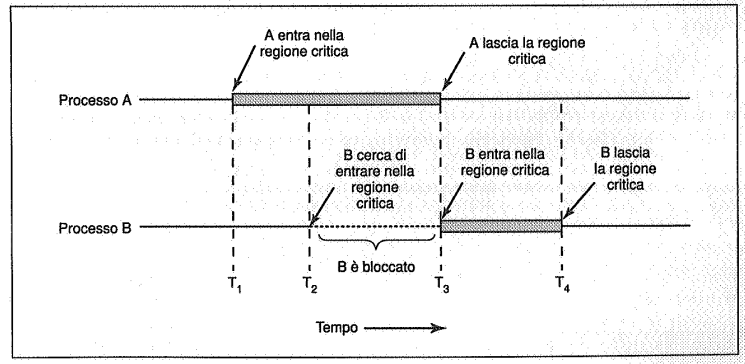
\includegraphics[width=1\linewidth]{assets/mutuaesclusione6.png}
    \caption{Il comportamento desiderato, mutua esclusione}
\end{figure}

\section{Mutua esclusione con attesa attiva}

\subsection{Disabilitazione degli interrupt}

La soluzione più semplice consiste nel permettere a ciascun processo di disabilitare le interruzioni non appena entra nella sua regione critica, e di riabilitarle non appena ne esce. Con le interruzioni disabilitate la CPU non può essere assegnata ad un altro processo.

Questa tecnica è spesso utile nel kernel ma è poco appropriata per i processi utente.


\subsection{Variabili di lock}
Supponiamo di avere una singola variabile condivisa (\textbf{di lock}), con valore iniziale 0. Quando un processo vuole entrare in regione critica controlla prima la variabile, se è 0 la imposta ad 1 ed entra, altrimenti aspetta.

Questa soluzione non è propriamente una soluzione in quanto può verificarsi lo stesso che due processi siano nelle loro sezioni critiche, basti pensare che la lettura della variabile di lock da parte di un processo, può essere immediatamente seguita dalla lettura della stessa da parte dell'altro processo, causando l'inevitabile.

\subsection{Alternanza stretta}

\begin{figure}[H]
    \centering
    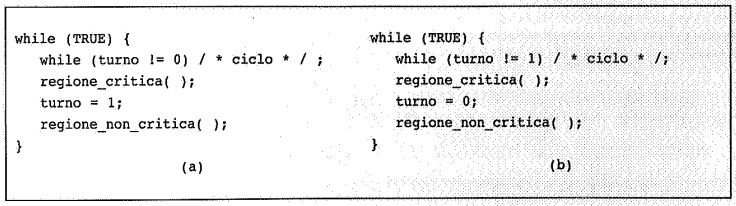
\includegraphics[width=1\linewidth]{assets/alternanzastretta6.png}
    \caption{(a) processo 0 (b) processo 1.}
    \label{alternanzastretta}
\end{figure}

Nell'approccio presentato in figura \ref{alternanzastretta} la variabile intera \textit{turno} tiene traccia del processo al quale tocca. 

Il testare continuamente una variabile, in attesa che essa assuma un certo valore, è detta \textbf{attesa attiva}, o \textit{busy waiting}. Di norma è una procedure che andrebbe evitata, visto l'incredibile spreco di CPU.
Un lock che usa l'attesa attiva è detto \textbf{spin lock}.

Questa soluzione è cattiva se uno dei due processi è molto più lento dell'altro. Inoltre anche questa non è una vera e propria soluzione: infatti essa viola la condizione 3 enunciata prima, il processo 0 è bloccato da un processo che non è nella sua sezione critica.

Pur non essendo una soluzione rappresenta una modalità, poco seria, di evitare qualsiasi corsa critica.

\subsection{La soluzione di Peterson}

\begin{figure}[H]
    \centering
    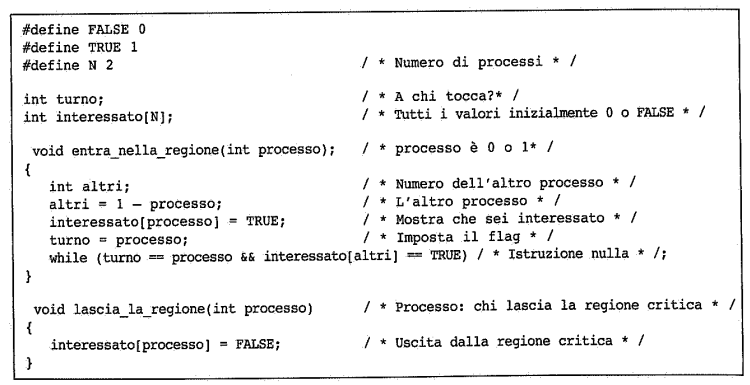
\includegraphics[width=1\linewidth]{assets/peterson6.png}
    \caption{La soluzione di Peterson}
    \label{peterson}
\end{figure}

L'algoritmo di Peterson è mostrato in figura \ref{peterson}.

Prima di entrare nella propria regione critica, ciascun processo chiama la funzione \textit{entra\_nella\_regione(id)} con il proprio identificativo. Invece per indicare che ha finito chiama \textit{lascia\_la\_regione(id)}, permettendo agli altri di entrare.

Consideriamo il caso peggiore: due processi chiamano \textit{entra\_nella\_regione(id)} quasi contemporaneamente. Ciò che succede è che il processo che la chiama per ultimo vedrà impostato il proprio \textit{id} nella variabile turno, quindi eseguirà la propria regione critica, mentre l'altro eseguirà il \textit{while} a vuoto finché il primo non libererà la risorsa.

\subsection{L'istruzione TSL}

Questa soluzione è una proposta hardware. I calcolatori progettati pensando ai processi multipli implementano un istruzione particolare:
\begin{verbatim}
    TSL RX,LOCK
\end{verbatim}
Test and Set Lock, verifica ed imposta il blocco: mette il contenuto della parola di memoria \textit{lock} nel registro \textit{rx}, e in seguito memorizza un valore diverso da 0 all'indirizzo di memoria di \textit{lock}. Queste due operazioni sono garantite indivisibili: nessun altro processore può accedere alla parola finché l'istruzione non è finita (essa è quindi un operazione \textbf{atomica}).

Per usare questa soluzione useremo una variabile condivisa, \textit{lock}, per coordinare l'accesso: quando essa è a 0 qualsiasi processo la può mettere ad 1 con \textit{TSL} e riportarla, in seguito all'esecuzione della sua regione critica, a 1 (usando una semplice istruzione \textit{move}).




\section{Sospensione e risveglio}

Tutte le soluzioni viste finora hanno un problema: l'attesa attiva. Possono anche venirsi a creare effetti inaspettati: se un processo \textit{a}, ad alta priorità, si trova nella sua regione critica, e uno \textit{b}, con priorità più bassa, passa nello stato \textit{ready}, il primo comincia l'attesa attiva, ma poiché \textit{b} non viene mai scelto quando \textit{a} è in esecuzione, \textit{a} non ha mai modo di lasciare la regione critica e \textit{b} cicla all'infinito. Questo è il \textbf{problema di inversione delle priorità}.

Vediamo alcune primitive di comunicazione tra processi che li bloccano, anziché sprecare tempo di CPU.

Una delle coppie più semplici è formata dalle primitive \textbf{sleep} e \textbf{wake up}: la prima provoca il blocco del processo chiamante, la seconda, tramite un parametro identificativo del processo in questione, lo risveglia. Esiste un'alternativa che specifica un parametro sia per \textit{sleep} che per \textit{wake up}, in modo da accoppiarle.

Per esprimere le chiamate di sistema corrispondenti le mostreremo come semplici chiamate a procedure di libreria in C. Non fanno parte della libreria standard, ma saranno presumibilmente disponibili in ogni sistema che le supporta.

Un classico problema che le coinvolge è una sveglia spedita ad un processo sveglio, in quel caso occorre aggiungere un \textbf{bit di attesa della sveglia} (wake up waiting bit), che non è altro che un salvadanaio per i segnali di sveglia. Questa semplice soluzione non basta per situazioni con \textit{n} processi.




\section{I semafori}
Dijkstra suggerì di usare una variabile intera per contare il numero di sveglie salvate per l'uso futuro. Nella sua proposta venne introdotto un nuovo tipo di variabile, chiamata \textbf{semaforo}: se esso ha valore 0 non è stata salvata alcuna sveglia, se ha un valore positivo una o più sveglie sono pervenute.

Vennero proposte due operazioni: 
\begin{enumerate}
    \item \textbf{down}, analoga di sleep: se il numero di sveglie è maggiore di zero viene decrementato di uno il valore; se è zero il processo viene sospeso, in attesa di completare la \textit{down}.
    \item \textbf{up}, analoga di wake up: incrementa il valore del semaforo di uno; se uno o più processi erano sospesi su quel semaforo ne viene scelto uno da fare ripartire (anche a caso).
\end{enumerate}

Controllare il valore, cambiarlo ed eventualmente sospendersi sono tutte operazioni eseguite in un'unica, indivisibile, \textbf{azione atomica}. Anche incremento semaforo e risveglio sono istruzioni indivisibili. Questa atomicità è essenziale.

\subsection{Produttore-Consumatore con semafori}

La soluzione è mostrata in figura \ref{producerconsumersemaphore}.
Normalmente \textit{up} e \textit{down} sono implementate come chiamate di sistema ed il sistema operativo, siccome sono operazioni da pochissime istruzioni, disabilita gli interrupt senza causare danni. Nel caso di CPU multiple il semaforo va protetto con TSL per garantire che solo una alla volta lo interroghi. 

\begin{figure}[H]
    \centering
    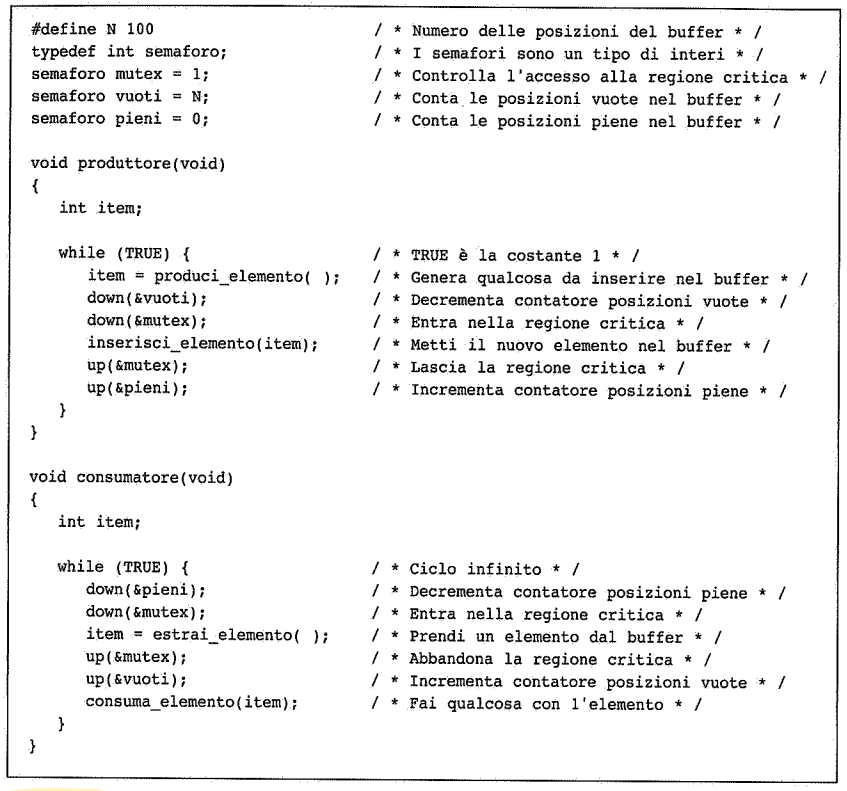
\includegraphics[width=1\linewidth]{assets/producerconsumersemaphore6.png}
    \caption{Produttore-Consumatore con semaforo.}
    \label{producerconsumersemaphore}
\end{figure}

La soluzione prevede l'utilizzo di tre semafori:
\begin{enumerate}
    \item \textit{pieni}: conta il numero di elementi che sono occupati. Inizialmente posto a zero.
    \item \textit{vuoti}: conta quelli vuoti. Inizialmente posto uguale al numero di elementi nel buffer.
    \item \textit{mutex}: garantisce che produttore e consumatore non accedano contemporaneamente al buffer. Inizialmente posto a uno.
\end{enumerate}

I semafori come \textit{mutex}, che vengono inizializzati ad uno e sono usati per organizzare la mutua esclusione di due processi, sono detti \textbf{semafori binari}.

È garantita la mutua esclusione se ogni processo chiama una \textit{down} prima di entrare nella sua regione critica, e una \textit{up} subito dopo esserne uscito.

I semafori \textit{pieni} e \textit{vuoti} invece sono semafori di \textbf{sincronizzazione}, garantiscono quindi che l'\textit{ordine} di alcune operazioni sia ben definito.




\section{Mutex}
Quando non è necessaria la caratteristica dei semafori di saper contare, ne viene utilizzata una versione semplificata, detta \textbf{mutex}. Sono usati per gestire la mutua esclusione, sono facili ed efficienti da implementare, vengono spesso usati per i thread implementati nello spazio utente (quando è prevista l'istruzione TSL).

Un \textit{mutex} è una variabile che può essere in due stati: bloccato e non bloccato. Occorre quindi un solo bit per rappresentarlo, anche se spesso si utilizza un intero (zero significa bloccato, non bloccato per ogni altro valore).

Vengono usate due procedure: 
\begin{enumerate}
    \item \textit{mutex lock}: simile a soluzioni già viste, ma con la sostanziale differenza che non implementa l'\textit{attesa attiva}, non ci sarebbe alcun clock a fermare i thread in esecuzione da troppo. Quando un thread fallisce nell'acquisizione di un blocco chiama la \textbf{thread\_yield}, per lasciare la CPU ad un altro thread (essa è una chiamata allo schedulatore non una di sistema).
    \item \textit{mutex\_unlock}: il nome è autoesplicativo. Inoltre, se più thread sono bloccati sul mutex, ne viene scelto uno a caso per acquisire la risorsa.
\end{enumerate}

Se i processi hanno spazio di indirizzamento separato, come abbiamo continuamente detto, come possono condividere la variabile turno dell'algoritmo di Peterson, o i semafori o un buffer comune? 

Ci sono due risposte. Primo, alcune delle strutture dati condivise, come i semafori, possono essere memorizzate nel kernel e accedute solo tramite chiamate di sistema e questo approccio elimina il problema. Secondo, la maggior parte dei sistemi operativi moderni (compresi UNIX e Windows) fornisce un modo attraverso il quale i processi possono condividere porzioni del loro spazio di indirizzamento con altri processi, così i buffer e altre strutture dati possono essere condivise. Nel caso peggiore, quando non è possibile nient'altro, può essere usato un file condiviso.




\section{Monitor}
La scrittura di programmi contenenti semafori è tutt'altro che banale.
Nel produttore-consumatore con semafori, se dovesse accadere che \textit{mutex} venga decrementato prima di \textit{vuoti} invece che dopo, se il buffer fosse completamente pieno, il produttore si bloccherebbe con \textit{mutex} a 0, a questo punto alla prossima down del consumatore entrambi i processi risulterebbero bloccati per sempre... questa situazione viene spesso indicata con \textbf{deadlock} (stallo).

Per rendere più semplice la scrittura di questi programmi venne introdotta una primitiva di sincronizzazione più ad alto livello, chiamata \textbf{monitor}.

Un monitor è una collezione di procedure, variabili e strutture dati che vengono raggruppate insieme in un tipo speciale di modulo o package. I processi possono chiamare le procedure del monitor ma non possono accedere alle strutture interne.

Essi possiedono un importante proprietà che li rende utili per ottenere la mutua esclusione: ad ogni istante, un solo processo può essere attivo in un monitor. Essendo essi un costrutto del linguaggio di programmazione il compilatore sa che devono essere trattati con cautela. Tipicamente, ogni volta che una procedura del monitor va attivata, prima di farlo si controlla che nessun'altra sia in esecuzione, in caso affermativo si fa partire la procedura richiesta.
Spetta quindi al compilatore implementare la mutua esclusione, sebbene sia un modo comune implementarla utilizzando un \textit{mutex}.

Per chi scrive i programmi, a questo punto, basta sapere che, trasformando tutte le sezioni critiche in procedure del monitor, due processi qualunque non potranno mai eseguire contemporaneamente le proprie sezioni critiche.

Occorre definire come bloccare i processi quando non possono proseguire.
La soluzione sta nell'introduzione di \textbf{condition variables}, con due operazioni associate: \textit{wait} e \textit{signal}. Quando una procedura scopre di non poter continuare chiama una wait su una qualche \textit{variabile di tipo condizione} (nell'esempio potrebbe essere la variabile \textit{pieni}). Un altro processo invece, quando vuole svegliare il partner sospeso, chiama una signal sulla stessa variabile.

Un ultima cosa da fare, per evitare che due processi siano nel monitor contemporaneamente dopo la signal, è definire cosa succede. Una scelta possibile è che chi chiama la signal debba istantaneamente uscire dal monitor.

Se viene eseguita una signal su una variabile su cui nessuno è sospeso, il segnale viene perso.

\subsection{Produttore-Consumatore con i monitor Java}

In Java, aggiungendo la parola chiave \textbf{synchronized} alla dichiarazione di un metodo, si garantisce che una volta che un thread ha iniziato l'esecuzione di quel metodo, a nessun altro thread sarà permesso di eseguire un metodo synchronized di quella stessa classe. Una soluzione al problema produttore-consumatore utilizzando i monitor in Java è mostrata in figura \ref{producerconsumermonitor}.

\begin{figure}[H]
    \centering
    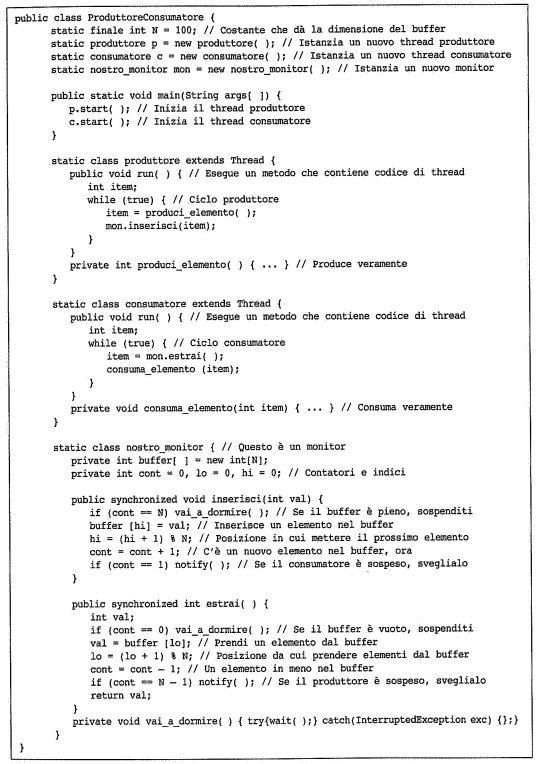
\includegraphics[width=1\linewidth]{assets/producerconsumermonitor6.png}
    \caption{Produttore-Consumatore con monitor.}
    \label{producerconsumermonitor}
\end{figure}

I metodi sincronizzati di Java differiscono in modo sostanziale dai monitor tradizionali: Java non ha variabili di tipo condizione, piuttosto due procedure, \textit{wait} e \textit{notify}, equivalenti di \textit{sleep} e \textit{wake up}, eccetto che, quando usate da metodi sincronizzati, non sono soggette a corse critiche.








\section{Lo scambio di messaggi}

La differenza tra le soluzioni proposte è che i semafori sono troppo a basso livello e di difficile gestione, e i monitor non sono utilizzabili in molti linguaggi di programmazione. Inoltre entrambe le soluzioni non permettono lo scambio di informazioni tra macchine.
Per quello è necessario qualcosa di diverso: \textbf{lo scambio di messaggi}.

Questo metodo di comunicazione tra processi usa due primitive:
\begin{verbatim}
    send(dest, &message);
    receive(source, &message);
\end{verbatim}

Esse sono chiamate di sistema, non costrutti del linguaggio, possono essere quindi inserite in procedure di libreria.

La prima spedisce un messaggio ad una destinazione. La seconda lo riceve da una determinata sorgente, o da \textit{ANY}. Se non è disponibile alcun messaggio il ricevente potrebbe bloccarsi fino all'arrivo di uno.

\subsection{Problematiche di progetto dei sistemi}
Se le macchine che comunicano stanno sulla rete i messaggi possono essere persi. Per prevenire che ciò sia fatale si potrebbe pensare ad un messaggio di \textbf{acknowledgement}, il quale, se non ricevuto in un tempo limite dal mittente, suggerisce a quest'ultimo il re-invio del messaggio.

Un altro problema riguarda l'\textbf{autenticazione}, altre volte sono un problema le prestazioni... insomma, questi sistemi sono soggetti a parecchie vulnerabilità a cui è necessario prestare attenzione.

\subsection{Produttore-Consumatore con scambio di messaggi}
Vediamo come può essere risolto il problema  con scambio di messaggi e senza memoria condivisa. Una soluzione è in figura \ref{producerconsumermessages}

\begin{figure}[H]
    \centering
    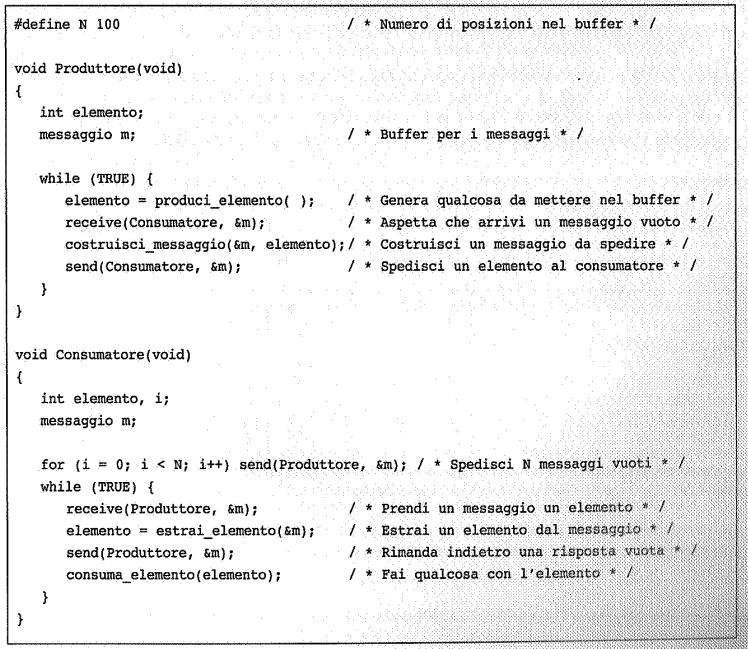
\includegraphics[width=0.7\linewidth]{assets/producerconsumermessages6.png}
    \caption{Produttore-Consumatore con N messaggi.}
    \label{producerconsumermessages}
\end{figure}

Un modo di indirizzare i messaggi è quello di assegnare ad ogni processo un indirizzo unico e di inviargli direttamente i messaggi. Un altro prevede di usare una nuova struttura dati, detta \textbf{mailbox}, che bufferizza uno specifico numero di messaggi. Nel secondo caso i parametri di \textit{send} e \textit{receive} sono mailbox e non processi. 

Quando un processo tenta di mandare un messaggio ad una mailbox piena esso viene sospeso finché non viene fatto spazio per il suo messaggio.

Un ultimo modo è il \textbf{rendez-vous}, esso è meno flessibile ma più facile da implementare: viene eliminata completamente la bufferizzazione, se la \textit{send} viene chiamata prima della \textit{receive} il mittente viene bloccato fino al sopraggiungere di quest'ultima; analogamente se la \textit{receive} è chiamata prima della \textit{send} è il destinatario a rimanere bloccato fino all'invio del messaggio.







\section{Barriere}
Un meccanismo di sincronizzazione per gruppi di processi. Alcune applicazioni sono divise in fasi e hanno la regola che nessun processo può proseguire finché tutti sono pronti per la fase successiva. Questo comportamento può essere ottenuto mediante una \textbf{barriera} alla fine di ogni fase: quando un processo la raggiunge viene bloccato finché tutti la raggiungono.

Un esempio è mostrato in figura \ref{barriere}.

\begin{figure}[H]
    \centering
    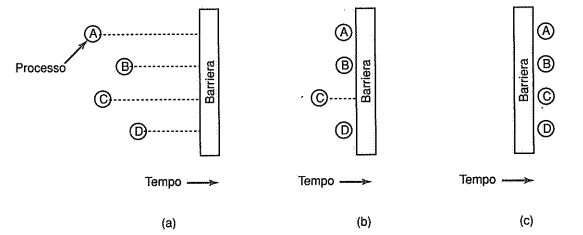
\includegraphics[width=0.7\linewidth]{assets/barriere6.png}
    \caption{Uso di una barriera.}
    \label{barriere}
\end{figure}

Il primo processo finisce i calcoli e chiama la primitiva \textit{barrier}, generalmente con una procedura di libreria, dopodiché viene sospeso. Quando anche l'ultimo processo chiama la primitiva tutti vengono liberati e si procede.

\subsection{CyclicBarrier di Java}
\dots


\subsection{CountDownLatch di Java}
\dots








\newpage
\section{Problemi classici di IPC}

\subsection{Filosofi a cena}
\textit{"Cinque filosofi sono seduti attorno ad un tavolo rotondo, ciascuno ha un piatto  di spaghetti e due forchette, posizionate a destra e sinistra rispetto al piatto; per mangiare il filosofo ha bisogno di entrambe le forchette; la vita dei filosofi si divide in periodi un cui pensano e periodi in cui mangiano. Quando un filosofo ha fame prende le forchette, mangia, ed in seguito depone le forchette e torna a pensare."}

\begin{figure}[H]
    \centering
    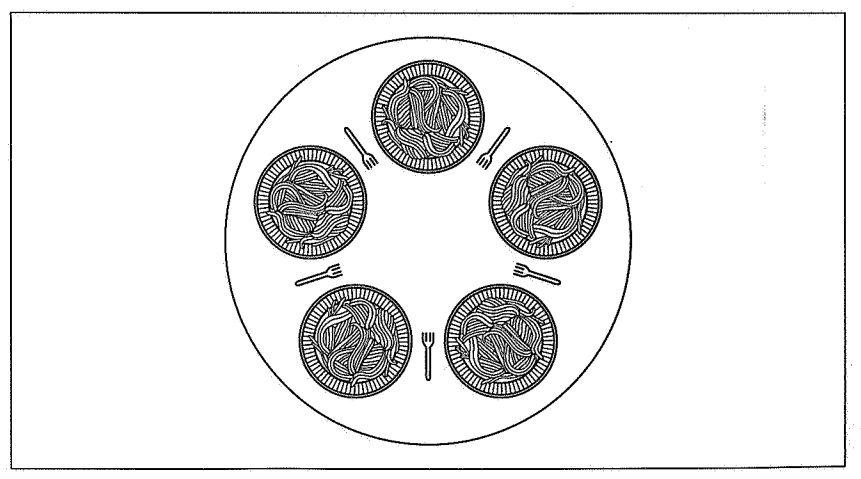
\includegraphics[width=0.5\linewidth]{assets/tavolofilosofi6.png}
    \caption{L'ora di cena al dipartimento di filosofia.}
\end{figure}

Occorre scrivere un programma che rappresenti tutti i filosofi, e che non si fermi mai.

Quello presentato è il famoso problema dei filosofi a cena. È utile per modellare processi che competono pr l'accesso esclusivo ad un numero limitato di risorse (come i dispositivi in/out).

\paragraph*{}
La soluzione banale non funziona, poiché se tutti i filosofi prendono contemporaneamente la forchetta non ne rimangono abbastanza e l'intero programma si blocca per sempre, senza fare progressi (una situazione di questo tipo è detta \textbf{starvation}). 

\paragraph*{}
Una popolare soluzione prevede di far attendere un piccolo tempo casuale al filosofo prima di ritentare a prendere le forchette. Tuttavia esistono situazioni estremamente delicate in cui non è possibile affidarsi a dei numeri casuali.

\paragraph*{}
Una prima soluzione, ancora non perfetta, prevede l'utilizzo di un semaforo binario: prima di prendere possesso delle forchette il filosofo chiama una \textit{down} su un mutex, dopo averle deposte invece ci chiama una \textit{up}. Questa soluzione non è ottimale in quanto è un solo filosofo alla volta a mangiare, se fosse ottimale con 5 forchette sono due i filosofi a poter mangiare in contemporanea.

\paragraph*{}
Una soluzione definitiva (Figura \ref{soluzionefilosofi}) usa un vettore \textit{affamato}, per tenere traccia se un filosofo sta mangiando, pensando o aspettando. In questo caso un filosofo si può portare nello stato in cui mangia solo se nessuno dei suoi vicini sta mangiando. Il programma usa un vettore di semafori, uno per filosofo, in modo tale da permettere ai filosofi di bloccarsi nel caso in cui debbano aspettare.

\begin{figure}[H]
    \centering
    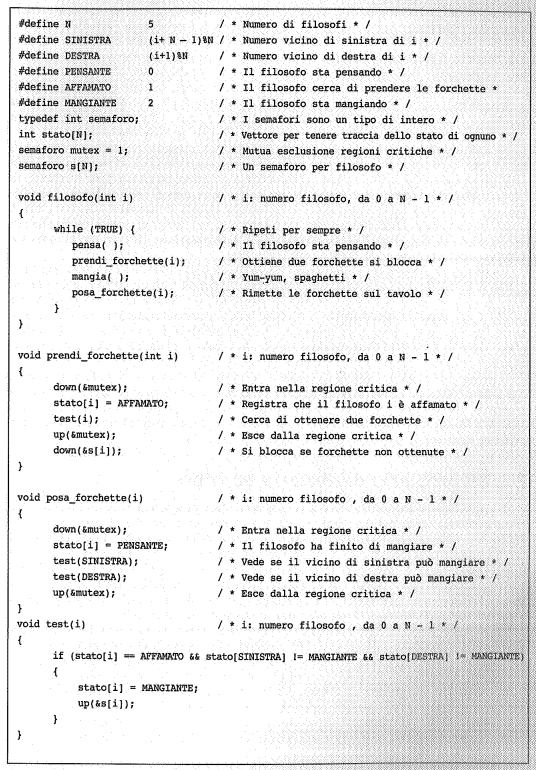
\includegraphics[width=1\linewidth]{assets/soluzionefilosofi6.png}
    \caption{Una soluzione ottimale al problema dei filosofi.}
    \label{soluzionefilosofi}
\end{figure}


\subsection{Lettori e scrittori}
Un altro problema noto è quello dei lettori e scrittori, che modella il problema di accesso ad una base di dati. Supponendo di avere \textit{n} processi che tentano di accedere ad un database dobbiamo fare in modo che sia i processi che scrivono che quelli che leggono possano competere in modo sano per la risorsa.

%cambia ref sotto qua
Una soluzione è mostrata in Figura \ref{soluzionelettoriscrittori}. In questo caso il primo lettore che ottiene l'accesso esegue una \textit{down} sul semaforo \textit{db}. I successivi lettori incrementano solamente un contatore, \textit{rc}, l'ultimo lettore che se ne va invece chiama la \textit{up}, permettendo all'eventuale scrittore bloccato di accedere. 

Questa strategia va KO se arrivano spesso lettori, è possibile che lo scrittore aspetti per sempre. Per ovviare si può fare in modo che un nuovo lettore che arriva si accodi agli scrittori in attesa, tuttavia anche questa soluzione presenta problemi di prestazioni. Esistono anche soluzioni che favoriscono gli scrittori.

\begin{figure}[H]
    \centering
    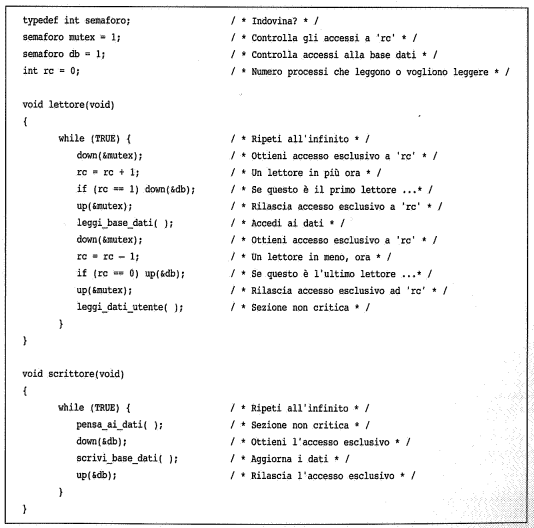
\includegraphics[width=1\linewidth]{assets/soluzionelettoriscrittori6.png}
    \caption{Una soluzione per il problema lettori e scrittori.}
    \label{soluzionelettoriscrittori}
\end{figure}


\subsection{Il barbiere che dorme (facoltativo)}

\textit{"Nel negozio c'è un barbiere, una sedia da lavoro e n sedie per far sedere i clienti in attesa. Se non ci sono clienti il barbiere si siede sulla sedia da lavoro e dorme. Quando arriva un cliente sveglia il barbiere. Se arrivano altri clienti mentre sta lavorando si siedono ad aspettare sulle n sedie, se sono tutte occupate il nuovo cliente se ne va."}

il problema in questo caso è programmare il barbiere ed i clienti senza arrivare ad avere corse critiche.

\begin{figure}[H]
    \centering
    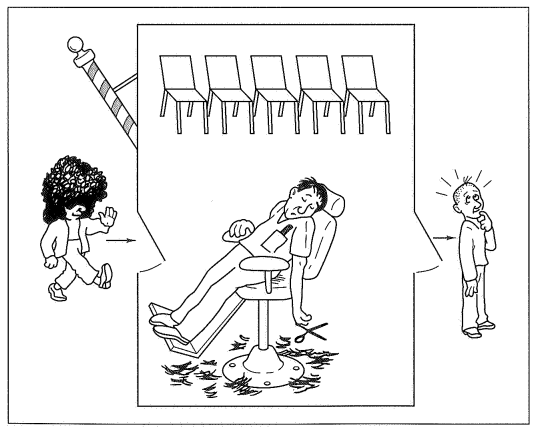
\includegraphics[width=0.5\linewidth]{assets/barbiere6.png}
    \caption{Un tipico barbiere del sud.}
\end{figure}


Una soluzione possibile usa tre semafori: \textit{clienti} che conta il numero dei clienti in attesa sulle sedie, \textit{barbieri} che conta il numero di barbieri (0 o 1) inattivi, e \textit{mutex} che viene usato per la mutua esclusione. Viene aggiunta una variabile copia di \textit{clienti} che permette ai nuovi clienti di leggere quanti sono ad aspettare (senza questa nuova variabile non ci sarebbe stato modo di leggere il semaforo). 

La mattina il barbiere esegue la procedura \textit{barbiere}, che lo blocca sul semaforo clienti, va quindi a dormire finché non arriva il primo cliente. Quando quest'ultimo arriva esegue la procedura \textit{cliente}, iniziando con l'acquisizione di \textit{mutex} per entrare in regione critica. In seguito controlla se il numero di clienti in attesa non riempie le sedie e, in caso negativo, rilascia \textit{mutex} e se ne va senza taglio di capelli. Se invece c'è posto incrementa la variabile \textit{in\_attesa}, esegue una \textit{up} su clienti, risvegliando il barbiere. Quando il cliente rilascia \textit{mutex} il barbiere gli taglia i capelli.

\begin{figure}[H]
    \centering
    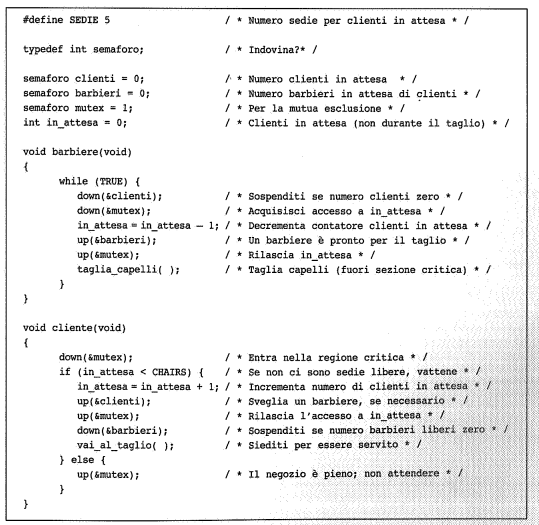
\includegraphics[width=0.5\linewidth]{assets/soluzionebarbiere6.png}
    \caption{Una soluzione per il problema del barbiere.}
\end{figure}
